%*******************************************************************************
%****************************** Second Chapter *********************************
%*******************************************************************************

\chapter{The Prototype Detector}\label{Chp:ThePrototypeDetector}

\ifpdf
    \graphicspath{{Chapter2/Figs/Raster/}{Chapter2/Figs/PDF/}{Chapter2/Figs/}}
\else
    \graphicspath{{Chapter2/Figs/Vector/}{Chapter2/Figs/}}
\fi


This thesis will cover two distinct versions of the detector. The original prototype detector which was re-purposed technology from the T2K ND280 ECal \cite{Allan_2013} and an upgraded version which uses the same basic materials in the detector but upgraded electronics and containment which will be refereed to as the ``Verification Instrument for Direct Assay of Nuclear Reactors at Range'' (VIDARR) detector. The rest of this section will focus on the prototype detector.
\\\\As it is the basis for the other detectors a quick overview of the T2K ND280 ECal will be required. The ND280 is series of detectors from the neutrino oscillation experiment T2K which relies on a $\mu_nu$ beam entering the detector as show in figure \ref{fig:nd280Fig}. This detector was comprised of several different types of detector including time projection chambers (TPCs) and fine-grained detectors (FGDs) and electromagnetic calorimeters (ECals) \cite{Allan_2013}. The ECals are of particular interest as they are the basis for the prototype and VIDARR detectors. 
\begin{figure}[htbp]
 \centering
 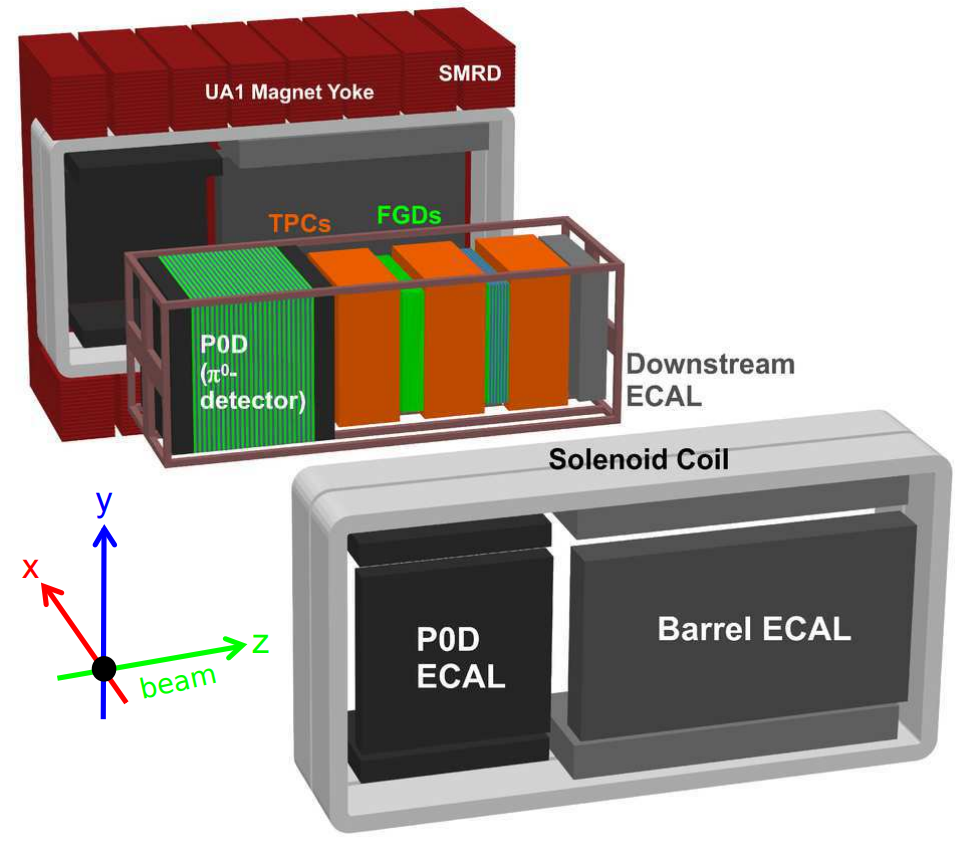
\includegraphics[width=\linewidth/2]{Chapter2/Figs/Raster/ND280Fig.png} 
 \captionof{figure}{Diagram of the ND280 detector. From \cite{Allan_2013}} %~can be used as a kind of place holder in latex
 \label{fig:nd280Fig}
\end{figure}
The T2K Ecals were made from plastic scintillating bars measuring 4\,cm by 1\,cm with varying lengths arranged in alternating layers at 90 degrees to each other \cite{Allan_2013}. Wavelength shifting (wls) fibres were placed in the centre of the scintillating bars which shift the wavelength from blue to green \cite{Allan_2013}. These wavelength shifting fibres are then connected to multi-pixel photon counters (MPPCs) which are the instrument which reads out the signal. This signal is then read in by Trip-T front-end electronic boards (TFBs) which then splits the signal into different cycles each containing 1.5 microseconds of information. All of this is shared by the prototype detector. 
\\\\However a crucial different between the ECals of the ND280 and the prototype detector is that the (ECals) had a layer of lead in between each of the plastic scintillating layers \cite{Allan_2013}. In the prototype this has been replaced with a layer of gadolinium so that neutrons were capture for inverse $\beta$ decay. The prototype was also designed to fit inside of a shipping container each bar having a length of 152\,cm and the whole detector measuring 152\,cm by 152\,cm with 49 layers of plastic scintillating bars totalling 49\,cm. The electronic systems were also adapted from the from the T2K system however they were altered such that they triggered on a gadolinium cascade from inverse $\beta$ decay. There were 23 cycles numbered from 0-22 with 0-17 cycles being considered "prompt" and cycle 18 is the trigger cycle. Cycles 19 -22 were left alone so that they could be compared in case time dependent issues arose from the altered system. Cycles 19-22 are useful for $\mu$ tomography as time dependent errors can arise from this adaptation of the electronics. 
\\\\The original detector was deployed at Wylfa power station in Anglesey Wales for an 18-month period. This run proved successful measuring the power on from the reactor to within good agreement to the measured reactor flux see figure \ref{fig:prototypeMeasumentFlux}. With a measured anti-neutrino rate of 172.1 $\pm$ 4.6 candidates per day when the reactor is off and 203.7 $\pm$ 19.6 when the reactor was on \cite{Carroll_2018}. Unfortunately due to cooling issues with the prototype the reactor shutdown was not observed. This is one of the main motivating factors behind the upgrade of the detector as the first generation MPPCs and reporposed electronics were susceptible to high levels of noise if the temperature was not carefully controlled. 
\begin{figure}[htbp]
 \centering
 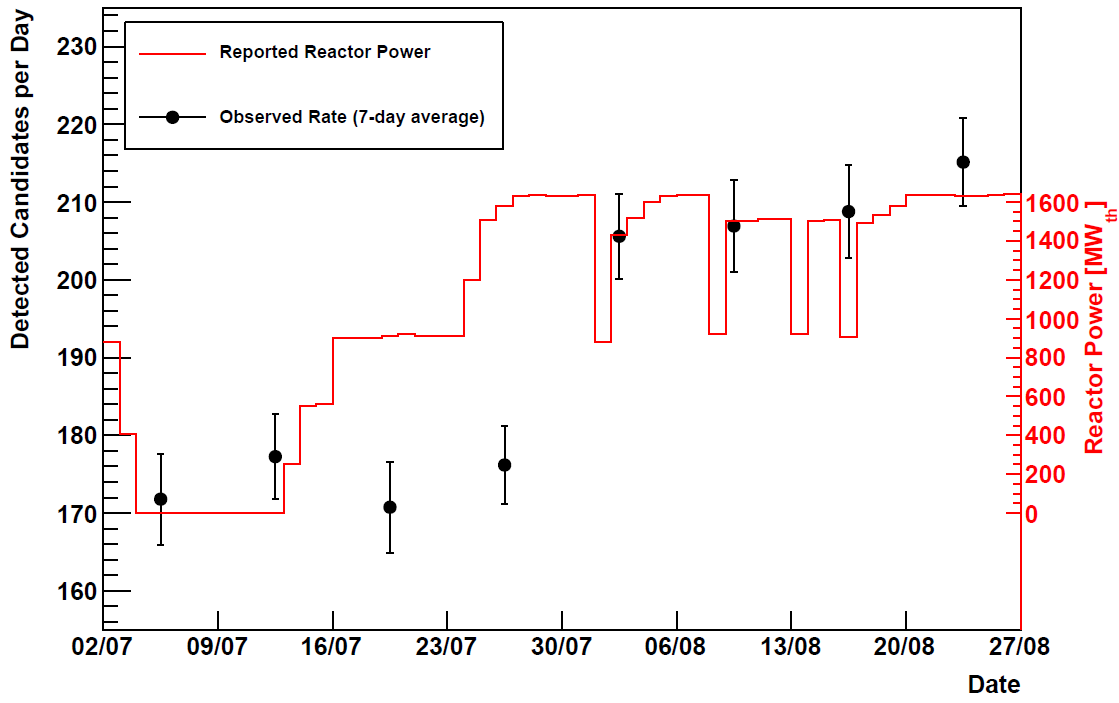
\includegraphics[width=0.90\linewidth]{Chapter2/Figs/Raster/prototypeMeasureOnFig.png} 
 \captionof{figure}{Measured anti-neutrino flux compared to the power generation from the Wylfa power station. From \cite{Carroll_2018}} %~can be used as a kind of place holder in latex
 \label{fig:prototypeMeasumentFlux}
\end{figure}

\section{Existing Reactor monitoring programs}\label{sec:exisitingReactorMonitoringPrograms}
%I feel like Double Chooz, Reno, KamLAND and Daya Bay are all very similar, liquid scintillating detectors with Gd doping initlally trying to find theta_13 but then transitioned to the 5 MeV reactor bump all of these are not proliforation focussed but measrument focussed experiments 
\subsection{Double Chooz}
%Double Chooz is probably one of the most well known reactor monitoring programs. \cite{abe2014improved} goes over some of the details and I have already mentioned it here. Also the \cite{lasserre2006} reference may be useful, used it once before in the first year literature survey. I've also cited \cite{Abe_2012} in the past and that may prove useful here. Further the reference \cite{Olive_2014} may also be of use. Double Chooz is a good one to cite because its clearly not in competition with VIDARR. It requires to be very close and a big hole dug underground and uses gadolinium suspended in liquid organic scintillator. Which is not cheap or portable, it does however give significantly better measurements for the disappearance of anti-neutrinos which the above references mention.
The Double Chooz experiment is an evolution of the original Chooz experiment which was set up at the Chooz nuclear power plant in France\cite{lasserre2006}. Both of these experiments attempted to measure the $\Bar{\nu_e}$ disappearance from the same reactor however the original Chooz experiment was unable to see any disappearance to a 90$\,\%$ confidence level \cite{Apollonio_2003}. Both experiments used gadolinium doped liquid scintillator with the Double Chooz experiment having a near and far detector at 280\,m and 1050\,m respectively\cite{lasserre2006}. Finally in 2012 $\Bar{\nu_e}$ disappearance was observed at the Double Chooz experiment \cite{Abe_2012}. These results were improved further in 2014 \cite{abe2014improved}.
\begin{figure}[htbp]
 \centering
 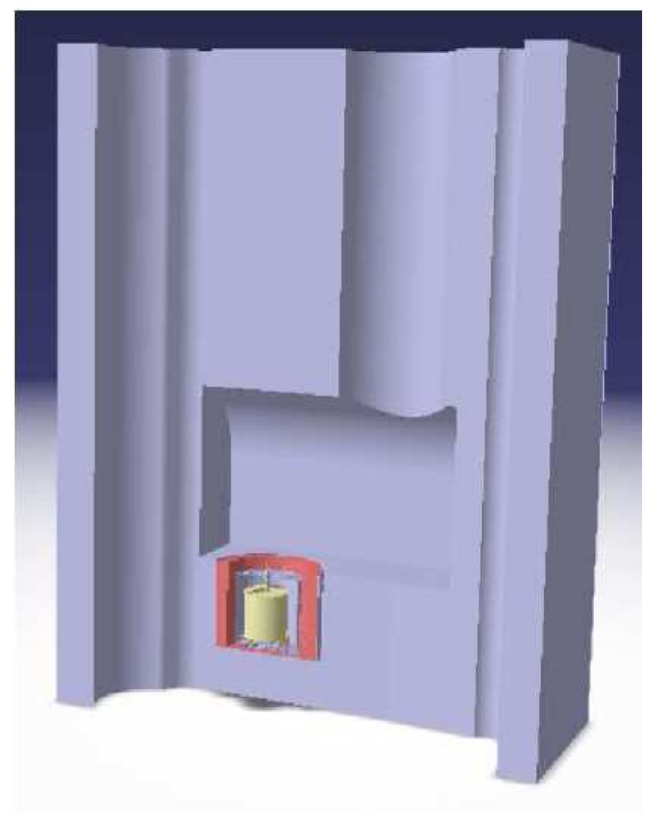
\includegraphics[height=75mm]{Chapter2/Figs/Raster/DCNearDetector.png} %height of this plot had to be adjusted because of its unusal diemensions
 \captionof{figure}{The near detector of the Double Chooz experiment 250\,m - 300\,m from the reactor with an overburden of 30\,m of rock \cite{lasserre2006}.} %~can be used as a kind of place holder in latex
 \label{DoubleChoozNearDetector}
\end{figure}
\\\\The Double Chooz experiment uses detector placed underground to allow for large amount of overburden to reduce background rates. As seen in figure \ref{DoubleChoozNearDetector} the overburden for the near detector is 30\,m\cite{lasserre2006}. The Double Chooz measurement  was not the first to measure the rate of $\Bar{\nu_e}$ disappearance \cite{reno_may_2012} it was able to produce a spectrum of the $\Bar{\nu_e}$ disappearance for $\theta_{13}$ which can be seen in \ref{doubleChoozSpectrumNoCaption}. The measured energy spectrum which can be seen as black points in figure \ref{doubleChoozSpectrumNoCaption}, the closest match to the data in the double Chooz data was found to the fitted red line with a $\sin^2{2\theta_{13}}$ = 0.109 $\pm$0.030(stat)$\pm$0.025(syst) as seen in figure \ref{doubleChoozSpectrumNoCaption} \cite{Abe_2012}. The data exclude the no-oscillation hypothesis at 99.8$\%$ CL (2.9$\sigma$)\cite{Abe_2012}. This data was further expanded upon in 2014 producing a result of $\sin^2{2\theta_{13}}$ = 0.090$^{+0.032}_{-0.029}$ using 467.90 live days of datat to within $3.0\sigma$ \cite{abe2014improved}.
\begin{figure}[htbp]
 \centering
 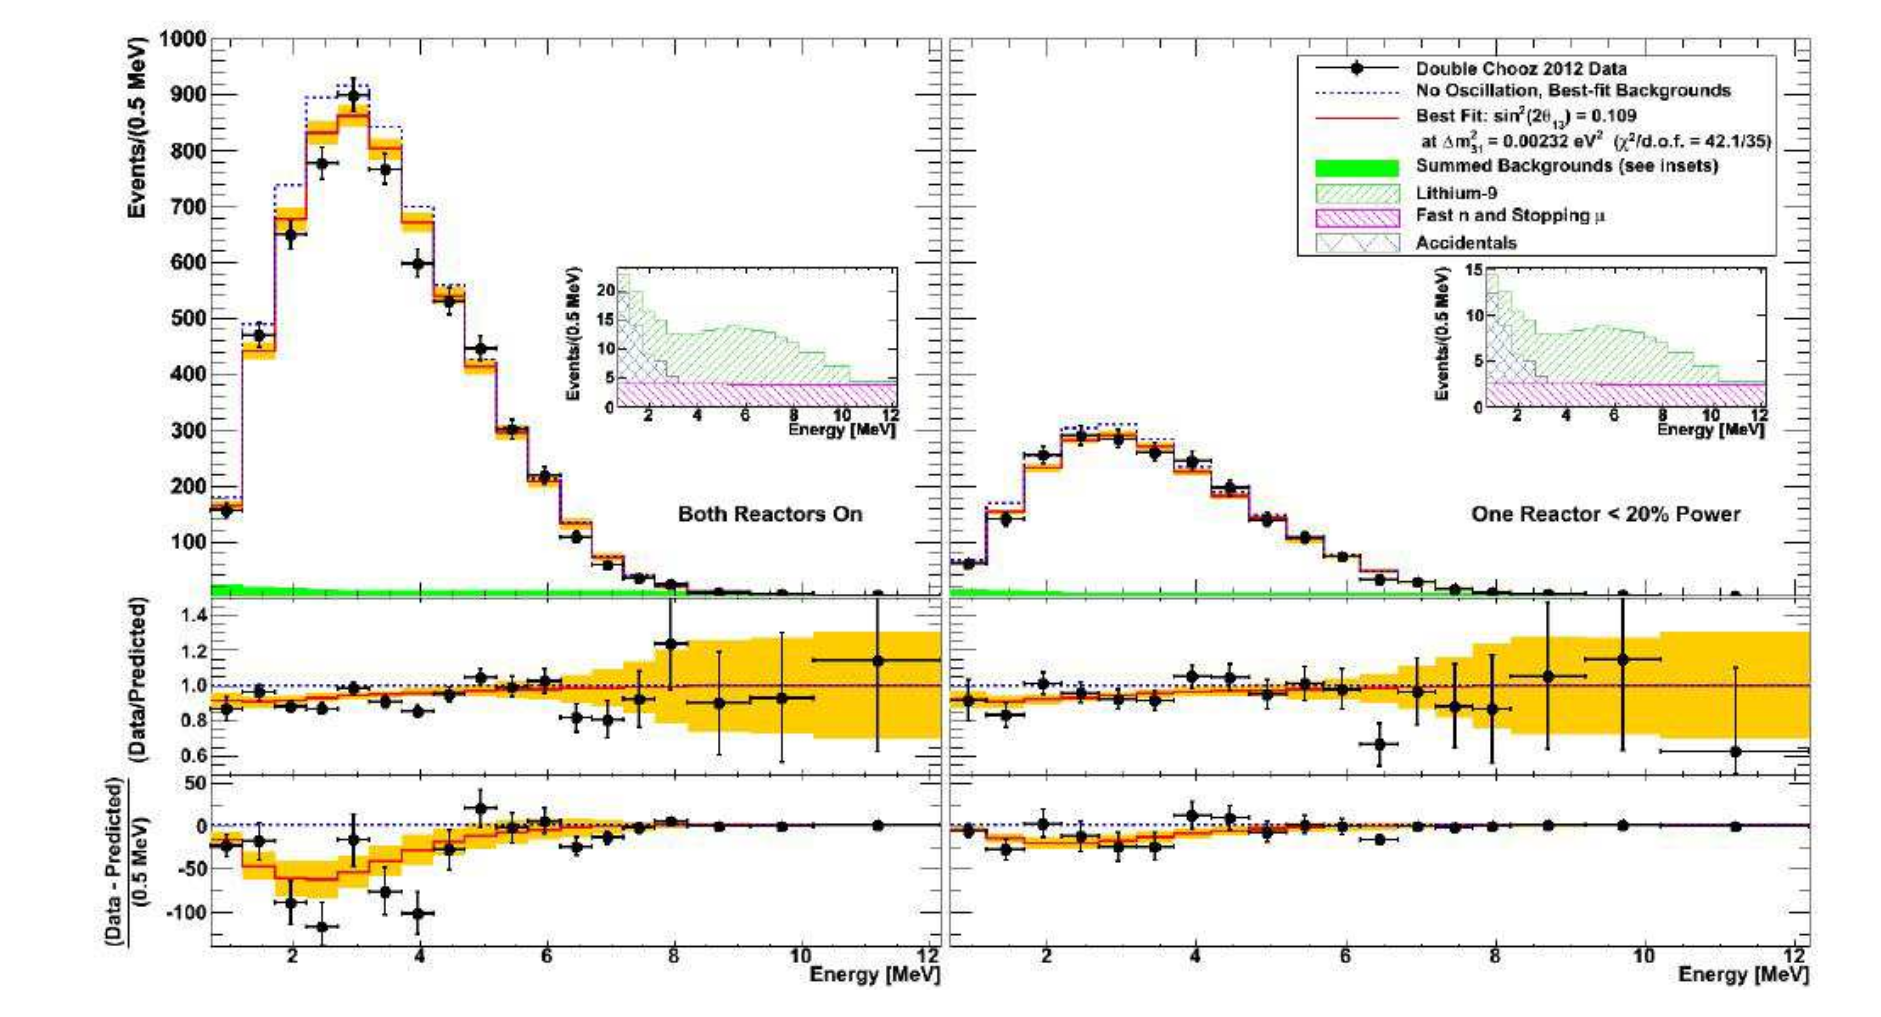
\includegraphics[width=\linewidth]{Chapter2/Figs/Raster/doubleChoozSpectrumNoCaption.png} %Just use linewidth for this one
 \captionof{figure}{Measured prompt energy spectrum for each integration period (data points) superimposed on the expected prompt energy spectrum, including backgrounds (green region), for the no-oscillation (blue dotted curve) and best-fit (red solid curve) at $\sin^2{2\theta_{13}}$ = 0.109 and $\Delta$m$^2_{31}$ = 2.32$\times$10$^{-3}$eV$^2$. Inset: stacked spectra of backgrounds. Bottom: differences between data and no-oscillation prediction (data points), and differences between best fit prediction and no-oscillation prediction (red curve).The orange band represents the systematic uncertainties on the best-fit prediction. From \cite{Abe_2012}} %~can be used as a kind of place holder in latex
 \label{doubleChoozSpectrumNoCaption}
\end{figure}
\subsection{RENO}
Papers found by this collaboration include \cite{reno_may_2012}, \cite{reno2013},  \cite{reno_may_2019}. Reno was the first collaboration to see $\Bar{\nu_e}$ disappearance \cite{Olive_2014} [CANNOT ACCESS CITATION AWAY FROM UNI, DOUBLE CHECK]. The RENO experiment consisted of two detectors 408.56\,m for the near detector,and 1443.99\,m for the far detector. A schematic of the detectors used in RENO can be seen in figure \ref{RENO_detector}, this detection system again uses Gd-doped liquid scintillator with PMTs. 
\begin{figure}[htbp]
 \centering
 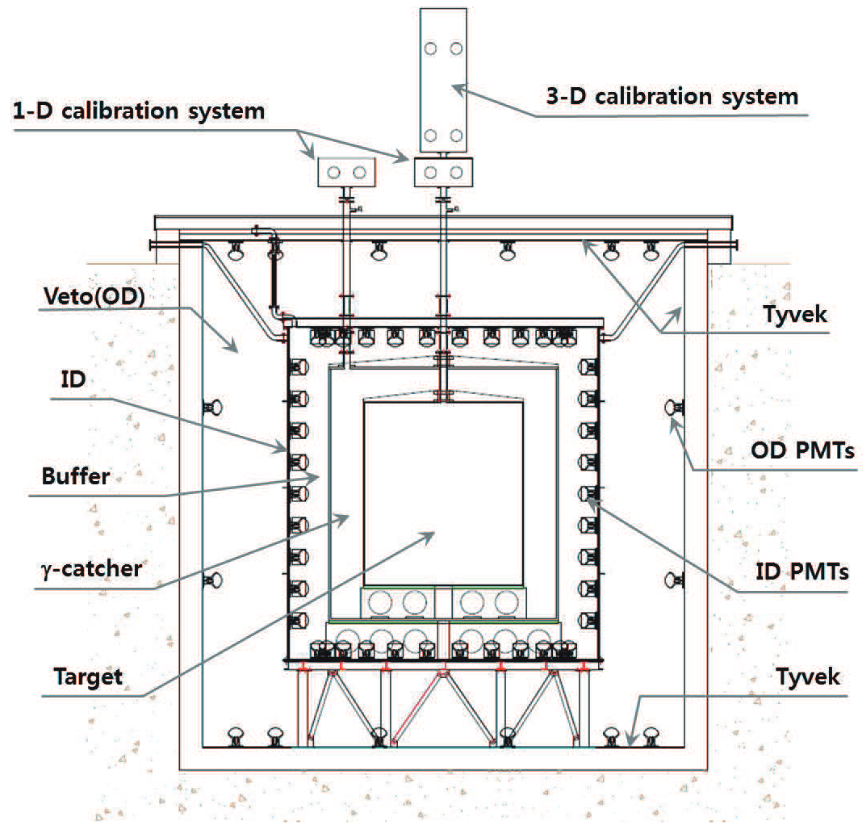
\includegraphics[width=0.5\linewidth]{Chapter2/Figs/Raster/RENO_detector.png} %Just use linewidth for this one
 \captionof{figure}{ schematic view of a RENO detector. The near and far detectors are identical. The detector seen in this figure consists of a main inner detector (ID) and an outer veto detector (OD) from \cite{reno_may_2012}} %~can be used as a kind of place holder in latex
 \label{RENO_detector}
\end{figure}
\\\\RENO's results in 2012 were consistent with neutrino oscillations to within 4.9 $\sigma$ from 6 2.8\,$GW_{th}$ reactors. The result from RENO in 2012 using a rate based analysis were $\sin^2{2\theta_{13}}$ = 0.113$\pm0.013$(stat.)$\pm0.019$(syst.) which was consistent with the findings that Double Chooz would produce later. These results were revised once again in 2013 using 800 days of live time to $\sin^2{2\theta_{13}}$ = 0.100 $\pm$ 0.010(stat) $\pm$ 0.015 (sys.) corresponding to 6.3 $\sigma$ significance \cite{reno2013}. The focus of the RENO collaboration has since shifted to analysing the 5\,MeV reactor anomaly \cite{reno_may_2019}.  
\subsection{DayaBay}
have this paper \cite{Daya_Bay_2017}, which was also mentioned in the RENO paper \cite{reno_may_2019} and there appears to be a detailed explanation of the experiment here \cite{DayaBay2007Precision}. It would appear to be very similar to RENO again an experiment that started off as a way to measure $\sin{\theta_{13}}$ and transitioned to analysing the 5\,MeV reactor bump.
\subsection{kamLand}
\subsection{WATCHMAN}
Designed with a similar goal to VIDARR but is far field as opposed to near field. Requires being buried underground similar to Double Chooz and is a water Cherenkov detector. And so is similar to super k and so referencing that would be a good approach. Also got the 2015 paper to pull from \cite{askins2015physics}. There's also steve dye's paper \cite{dye2017evaluating}. As well jon burns paper \cite{burns2018remote}. It may also be a good idea to cite the following \cite{danielson2019directionally} as its a summary talking about the use of anti-neutrinos for reactor non-proliferation.  
\subsection{Nucifier}
Makes sense to open with this found a paper from 2016 discussing their results \cite{nucifer2016}. Nucifier is a scaled down version of DoubleChooz, Daya Bay ect. Gd Doped liquid scintillator 
\subsection{SOLID}
\subsection{Chandler}
\subsection{PANDAS}
\subsection{PROSPECT}
